%%% The main file. It contains definitions of basic parameters and includes all other parts.

%% Settings for single-side (simplex) printing
% Margins: left 40mm, right 25mm, top and bottom 25mm
% (but beware, LaTeX adds 1in implicitly)
\documentclass[12pt,a4paper]{report}
\setlength\textwidth{145mm}
\setlength\textheight{247mm}
\setlength\oddsidemargin{15mm}
\setlength\evensidemargin{15mm}
\setlength\topmargin{0mm}
\setlength\headsep{0mm}
\setlength\headheight{0mm}
% \openright makes the following text appear on a right-hand page
\let\openright=\clearpage

%% Settings for two-sided (duplex) printing
% \documentclass[12pt,a4paper,twoside,openright]{report}
% \setlength\textwidth{145mm}
% \setlength\textheight{247mm}
% \setlength\oddsidemargin{14.2mm}
% \setlength\evensidemargin{0mm}
% \setlength\topmargin{0mm}
% \setlength\headsep{0mm}
% \setlength\headheight{0mm}
% \let\openright=\cleardoublepage

%% Generate PDF/A-2u
\usepackage[a-2u]{pdfx}

%% Character encoding: usually latin2, cp1250 or utf8:
\usepackage[utf8]{inputenc}

%% Prefer Latin Modern fonts
\usepackage{lmodern}

%% Further useful packages (included in most LaTeX distributions)
\usepackage{amsmath}        % extensions for typesetting of math
\usepackage{amsfonts}       % math fonts
\usepackage{amsthm}         % theorems, definitions, etc.
\usepackage{bbding}         % various symbols (squares, asterisks, scissors, ...)
\usepackage{bm}             % boldface symbols (\bm)
\usepackage{graphicx}       % embedding of pictures
\usepackage{fancyvrb}       % improved verbatim environment
\usepackage{natbib}         % citation style AUTHOR (YEAR), or AUTHOR [NUMBER]
\usepackage[nottoc]{tocbibind} % makes sure that bibliography and the lists
			    % of figures/tables are included in the table
			    % of contents
\usepackage{dcolumn}        % improved alignment of table columns
\usepackage{booktabs}       % improved horizontal lines in tables
\usepackage{paralist}       % improved enumerate and itemize
\usepackage{xcolor}         % typesetting in color

\usepackage{todonotes}

%%% Basic information on the thesis

% Thesis title in English (exactly as in the formal assignment)
\def\ThesisTitle{Searching Image Collections Using Deep Representations of Local Regions}

% Author of the thesis
\def\ThesisAuthor{Jana Bátoryová}

% Year when the thesis is submitted
\def\YearSubmitted{2020}

% Name of the department or institute, where the work was officially assigned
% (according to the Organizational Structure of MFF UK in English,
% or a full name of a department outside MFF)
\def\Department{Department of Software Engineering}

% Is it a department (katedra), or an institute (ústav)?
\def\DeptType{Department}

% Thesis supervisor: name, surname and titles
\def\Supervisor{RNDr. Jakub Lokoč, Ph.D.}

% Supervisor's department (again according to Organizational structure of MFF)
\def\SupervisorsDepartment{Department of Software Engineering}

% Study programme and specialization
\def\StudyProgramme{Computer Science}
\def\StudyBranch{Artificial Intelligence}

% An optional dedication: you can thank whomever you wish (your supervisor,
% consultant, a person who lent the software, etc.)
\def\Dedication{%
Dedication.
}

% Abstract (recommended length around 80-200 words; this is not a copy of your thesis assignment!)
\def\Abstract{%
Abstract.
}

% 3 to 5 keywords (recommended), each enclosed in curly braces
\def\Keywords{%
{key} {words}
}

%% The hyperref package for clickable links in PDF and also for storing
%% metadata to PDF (including the table of contents).
%% Most settings are pre-set by the pdfx package.
\hypersetup{unicode}
\hypersetup{breaklinks=true}

% Definitions of macros (see description inside)
%%% This file contains definitions of various useful macros and environments %%%
%%% Please add more macros here instead of cluttering other files with them. %%%

%%% Minor tweaks of style

% These macros employ a little dirty trick to convince LaTeX to typeset
% chapter headings sanely, without lots of empty space above them.
% Feel free to ignore.
\makeatletter
\def\@makechapterhead#1{
  {\parindent \z@ \raggedright \normalfont
   \Huge\bfseries \thechapter. #1
   \par\nobreak
   \vskip 20\p@
}}
\def\@makeschapterhead#1{
  {\parindent \z@ \raggedright \normalfont
   \Huge\bfseries #1
   \par\nobreak
   \vskip 20\p@
}}
\makeatother

% This macro defines a chapter, which is not numbered, but is included
% in the table of contents.
\def\chapwithtoc#1{
\chapter*{#1}
\addcontentsline{toc}{chapter}{#1}
}

% Draw black "slugs" whenever a line overflows, so that we can spot it easily.
\overfullrule=1mm

%%% Macros for definitions, theorems, claims, examples, ... (requires amsthm package)

\theoremstyle{plain}
\newtheorem{thm}{Theorem}
\newtheorem{lemma}[thm]{Lemma}
\newtheorem{claim}[thm]{Claim}

\theoremstyle{plain}
\newtheorem{defn}{Definition}

\theoremstyle{remark}
\newtheorem*{cor}{Corollary}
\newtheorem*{rem}{Remark}
\newtheorem*{example}{Example}

%%% An environment for proofs

\newenvironment{myproof}{
  \par\medskip\noindent
  \textit{Proof}.
}{
\newline
\rightline{$\qedsymbol$}
}

%%% An environment for typesetting of program code and input/output
%%% of programs. (Requires the fancyvrb package -- fancy verbatim.)

\DefineVerbatimEnvironment{code}{Verbatim}{fontsize=\small, frame=single}

%%% The field of all real and natural numbers
\newcommand{\R}{\mathbb{R}}
\newcommand{\N}{\mathbb{N}}

%%% Useful operators for statistics and probability
\DeclareMathOperator{\pr}{\textsf{P}}
\DeclareMathOperator{\E}{\textsf{E}\,}
\DeclareMathOperator{\var}{\textrm{var}}
\DeclareMathOperator{\sd}{\textrm{sd}}

%%% Transposition of a vector/matrix
\newcommand{\T}[1]{#1^\top}

%%% Various math goodies
\newcommand{\goto}{\rightarrow}
\newcommand{\gotop}{\stackrel{P}{\longrightarrow}}
\newcommand{\maon}[1]{o(n^{#1})}
% \newcommand{\abs}[1]{\left|{#1}\right|}
\newcommand{\dint}{\int_0^\tau\!\!\int_0^\tau}
\newcommand{\isqr}[1]{\frac{1}{\sqrt{#1}}}

%%% Various table goodies
\newcommand{\pulrad}[1]{\raisebox{1.5ex}[0pt]{#1}}
\newcommand{\mc}[1]{\multicolumn{1}{c}{#1}}


% Title page and various mandatory informational pages
\begin{document}
%%% Title page of the thesis and other mandatory pages

%%% SPECIMEN
%%% Inscriptions at the opening page of the hard cover

\pagestyle{empty}
\hypersetup{pageanchor=false}
\XXX{Opening page of the hard cover. Not a part of the electronic version.}
\begin{center}

\large
Charles University

\medskip

Faculty of Mathematics and Physics

\vfill

{\huge\bf BACHELOR THESIS}

\vfill

\hbox to \hsize{\YearSubmitted\hfil \ThesisAuthor}

\end{center}

\newpage\openright

%%% NEMICEPS

%%% Title page of the thesis

\pagestyle{empty}
\hypersetup{pageanchor=false}
\begin{center}

\centerline{\mbox{
\includegraphics[width=166mm]{img/logo-en.pdf}}}

\vspace{-8mm}
\vfill

{\bf\Large BACHELOR THESIS}

\vfill

{\LARGE\ThesisAuthor}

\vspace{15mm}

{\LARGE\bfseries\ThesisTitle}

\vfill

\Department

\vfill

{
\centerline{\vbox{\halign{\hbox to 0.45\hsize{\hfil #}&\hskip 0.5em\parbox[t]{0.45\hsize}{\raggedright #}\cr
Supervisor of the bachelor thesis:&\Supervisor \cr
\noalign{\vspace{2mm}}
Study programme:&\StudyProgramme \cr
\noalign{\vspace{2mm}}
Study branch:&\StudyBranch \cr
}}}}

\vfill

% Zde doplňte rok
Prague \YearSubmitted

\end{center}

\newpage

%%% NOPHD
%%% Here should be a bound sheet included -- a signed copy of the "bachelor
%%% thesis assignment". This assignment is NOT a part of the electronic
%%% version of the thesis. DO NOT SCAN.
\XXX{Bound into the introductory part must be the form with signed approval of the thesis topic (a photocopy suffices).
This is not a~part of the electronic version of the thesis, do not scan!}
%%% PHDNO

%%% A page with a solemn declaration to the bachelor thesis

\openright
\hypersetup{pageanchor=true}
\pagestyle{plain}
\pagenumbering{roman}
\vglue 0pt plus 1fill

\noindent
I declare that I carried out this bachelor thesis independently, and only with the cited
sources, literature and other professional sources. It has not been used to obtain another
or the same degree.

\medskip\noindent
I understand that my work relates to the rights and obligations under the Act No.~121/2000 Sb.,
the Copyright Act, as amended, in particular the fact that the Charles
University has the right to conclude a license agreement on the use of this
work as a school work pursuant to Section 60 subsection 1 of the Copyright~Act.

\vspace{10mm}

\hbox{\hbox to 0.5\hsize{%
In \hbox to 6em{\dotfill} date \hbox to 6em{\dotfill}
\hss}\hbox to 0.5\hsize{\dotfill\quad}}
\smallskip
\hbox{\hbox to 0.5\hsize{}\hbox to 0.5\hsize{\hfil Author's signature\hfil}}

\vspace{20mm}
\newpage

%%% Dedication

\openright

\noindent
\Dedication

\newpage

%%% Mandatory information page of the thesis

\openright

\vbox to 0.5\vsize{
\setlength\parindent{0mm}
\setlength\parskip{5mm}

Title:
\ThesisTitle

Author:
\ThesisAuthor

\DeptType:
\Department

Supervisor:
\Supervisor, \SupervisorsDepartment

Abstract:
\Abstract

Keywords:
\Keywords

\XXX{This information must be stored as PDF meta-data, too. Please refer to the {\tt README} file.}
\vss}

\newpage

\openright
\pagestyle{plain}
\pagenumbering{arabic}
\setcounter{page}{1}


%%% A page with automatically generated table of contents of the master thesis

\tableofcontents

%%% Each chapter is kept in a separate file
\chapter*{Introduction}
\addcontentsline{toc}{chapter}{Introduction}

In the last decades, we have witnessed a massive jump in the amount of digital information owned by individuals. Looking back 20-30 years, people used to record only a few hours of their lives, capturing precious moments. Now, according to available estimates, more than 500 hours of videos is uploaded every minute  to YouTube\footnote{\href{https://www.statista.com/statistics/259477/hours-of-video-uploaded-to-youtube-every-minute/}{Statista -- Hours of video uploaded to YouTube every minute}} only. Furthermore, decreasing prices and increasing availability of the recording electronics (especially smartphones) contribute to the amount of multimedia data created every day. It has also become a trend to share videos from day-to-day lives.

The significant increase in the volume of multimedia data opens several new challenges. One of the most vital is the need for effective search and retrieval. This problem is not only attractive to researchers, but the initiative also comes from the industry. Companies try to help their customers to organize a vast amount of multimedia data (Google Photos, Facebook, OneDrive, MEGA, and others). Those companies often rely on a broad spectrum of techniques used to store and organize the data internally. Unfortunately, users are usually provided with only the most straightforward technique to filter the data.

Besides attempting to overcome the challenges of querying large volumes of stored data, we will focus on a challenging scenario in which a user searches for one given image in a dataset. This task of searching for a previously seen multimedia object is often referred to as visual known-item search (\acrshort{kis}). In this thesis, we investigate several known-item search techniques where users provide a few example images as a collage query or browse through images of faces organized in a grid with respect to their similarity.

Known-item search has become a well-known research area \citep{8352047}. According to recent findings \citep{9037125}, most of the known-item search engines incorporate both querying and interactive search functionality. In order to elevate the level of developed KIS systems, researchers organize and participate in annual competitions. These efforts help to increase the interest in user-centered multimedia search. One, for example, is Video Browser Showdown\footnote{\url{https://videobrowsershowdown.org/}}, or shortly VBS. For a comparison, TRECVid \citep{2019trecvidawad} is also an annual competition with the main focus on ranking of scenes based on a textual description.

In this thesis, we investigate a couple of approaches to solve the known-item search task:

\begin{enumerate}
  \item Searching by an image collage query.
  \item Searching by browsing in a set of faces from the dataset.
\end{enumerate}

In the first approach, we focus on searching known images via only example images and their approximate position in the searched image. Users can create a collage of images that reminds them of the searched scene and then browse through the ranked result list looking for the match.

The second approach is an experimental test of the possibility of visual traversing through a dataset of faces. To present a user with a feasible amount of faces in one display, we tackle this challenge by organizing the faces into multilevel view supporting navigational queries. We implemented the traversal system, although we found out that this technique is less effective than other retrieval techniques presented in this thesis.

The goal of this thesis is to create a framework to test both approaches, as mentioned earlier. We aim to create a novice-friendly interface for smooth user-system interaction.

For the techniques which searching by the collages, We provide evaluations on an annotated set of queries. We manually created a set of collages, as our queries. We use them to test different hyperparameters of the proposed system. We evaluate the proposed methods based on the rank of the target image. Well-performing methods bring the searched items to the foreground, placing them at the top ranks.

We evaluate the second approach -- search based on faces -- with the help of a case study. We firstly investigate the space of the feature vectors by evaluating the responses from the survey. Then we present the solution. In the end, we provide a comparison between the average time needed to find a target face. We compare our traversal system to a display of randomly ordered faces.

\subsubsection*{Thesis structure}
The thesis is divided into four main chapters. After the Introduction, we continue by reviewing Related Work (\autoref{ch:related_work}) and Content-based image retrieval (\autoref{ch:preliminaries}). Related Work previews several existing frameworks for solving the KIS task. Content-based image retrieval chapter contains some elementary theoretical background for CBIR tasks and also evaluation settings.

After these introductory chapters, we present investigated approaches in chapters \ref{ch:object_location} and \ref{ch:face_search}. \todo{ref}

The end of the thesis is dedicated to the implementation of the aforementioned approaches. This includes the user's guide -- how to interact with the system, and developer's guide -- how to modify the dataset or how to incorporate a new approaches.

\bigskip

In summary, we designed and successfully tested a promising approach based on collage queries. The most promising approach splits images into multiple parts. We also developed a traversal system for previewing a dataset of faces. The experiments show, that using it decreased time of the individual search by XX\% \todo{}.
\chapter{Related work}
\label{ch:related_work}


This chapter reviews approaches made towards handling Known-item Search (KIS) task and the recent approaches for user-friendly traverse through the immersive amount of the visual data.

In recent years, we witnessed a significant advancement in the solution for the KIS task. The scale of the solution's complexity for user interaction ranges from simple ones (e.g., sketching color blocks) with only a few descriptors to the ones which use recent advance in deep learning, as for concept labeling (i.e, naming objects).

Our goal is to perform known-item-search task on a set of videos. We perform a common simplification, replacing videos with the set of images. We do this, since we look for a particular scene, which can be also an image. This level of abstraction therefore corresponds to the searched query. Also, this allows us to use a potential of a common neural networks and other solutions presented for 2D data (images in our case). For this task we perform sampling over the videos. More information is available in section \ref{}\todo{fix}, where more details about the dataset are available.

\section*{Known-item-search Task}

Known-item-search task is present in many different situations. The tasks is to efficiently retrieve a known item in the dataset. For example, for a database of newspaper article we may use such retrieval tools to find a particular article we are interested in. Our thesis focuses on visual KIS task, specifically we retrieve images. For the setting we solve our task in exist even annual competitions to share the knowledge and the advancements. One of such is Video Browser Showdown \ref{}\todo{fix}, which is taking place since 2012. We review a few of the presented solutions to this task from the last VBS2019. We mainly follow the summarization in the \ref{}\todo{fix}

The most common approach at the VBS2019 were "Query by an Image" and "Concept Labeling". Query by an image, in this case, mostly refers to finding the most similar results from databse to given image. The downside of this approach is mainly the difficulty to obtain an image, which would be sufficiently similar to the searched one.

The second most used approach at VBS2019 was Concept Labelling. In this case, a user can describe the scene using the words. The database is pre-annotated with the vocabulary of present items. During the request, the algorithm checks the database for the presence of the searched concept. This approach has a limitation of the vocabulary size. Recent advancement in the textual annotation neural networks is nowadays able to describe thousands of different objects by words, but still, this may present on the limitation on rarely used objects or hard to describe objects.

One of the approaches presented and used is by creating a color sketch. The user colors the canvas with respect to the original searched scene. The database is then traversed on the correspondence of the colors to the particular part of the image. We see a significant advantage of this approach to distinguish between the key objects in the scene spatially.
 
Solving KIS task in VBS setting offers the option of using full video information and not only snapshots. This approach enhances the possibilities spectrum to Temporal Queries or Multimodal queries. Also, the solution included Optical Character Recognition (OCR) was presented. We present our solution as a possible enhancement of a complex system in order to create multiple search strategies based on user-preference. 

\section*{Traversion Approaches}

Since the KIS task is the task of two sides -- the algorithm and the user, it is essential to not forget about the easy to use interface. A good overview of the dataset may hide some deficiencies of the algorithm so that the user can still find the search scene. As the  (Evaluation of VBS ref)\todo{fix} shows, the most common approach is to show a 2D grid of images to the user. Several approaches also provide an easy way to play the original video as one of the most immersive ways we have encountered to traverse a grid of images is placing these images on the globe with the possibility of multiway traversing (TODO: ref). We aim to achieve a similar level of smooth traversing.

The traversing systems rely on effective visualization techniques on high-number feature spaces. These systems create mostly a 2D grid of the images based on the distance between the samples in high dimensionality space. Though, this high dimensionality space, often produced by neural networks, may not have feasible representation in 2D space based on the hidden features. This is often caused by a lack of understanding and representability of the deep features. We aim to test this feature reduction to the 2D test in our face experiment with the use of deep neural network features.

\section{Existing systems}

In the next section we shortly investigate on existing frameworks, which competed in the Video Browser Showdown.

\subsection{VIRET}

A framework named VIRET (\cite{lokovc2019framework, lokovc2019viret}) is successfully participating in the competitions for a several years now. The framework evolved in the years and now it offers a wide variety of the strategies for solving KIS task. VIRET also implements own strategy for a frame selection, which we also used for obtaining our images. As one of the biggest strategical advantages of the VIRET we consider a multi-modal queries with relevance scores and update of the queries based on the results. We take VIRET as our inspiration and we do not implement the same approaches as are already present in the VIRET. We focus on testing new alternatives.

\begin{figure}
    \centering
    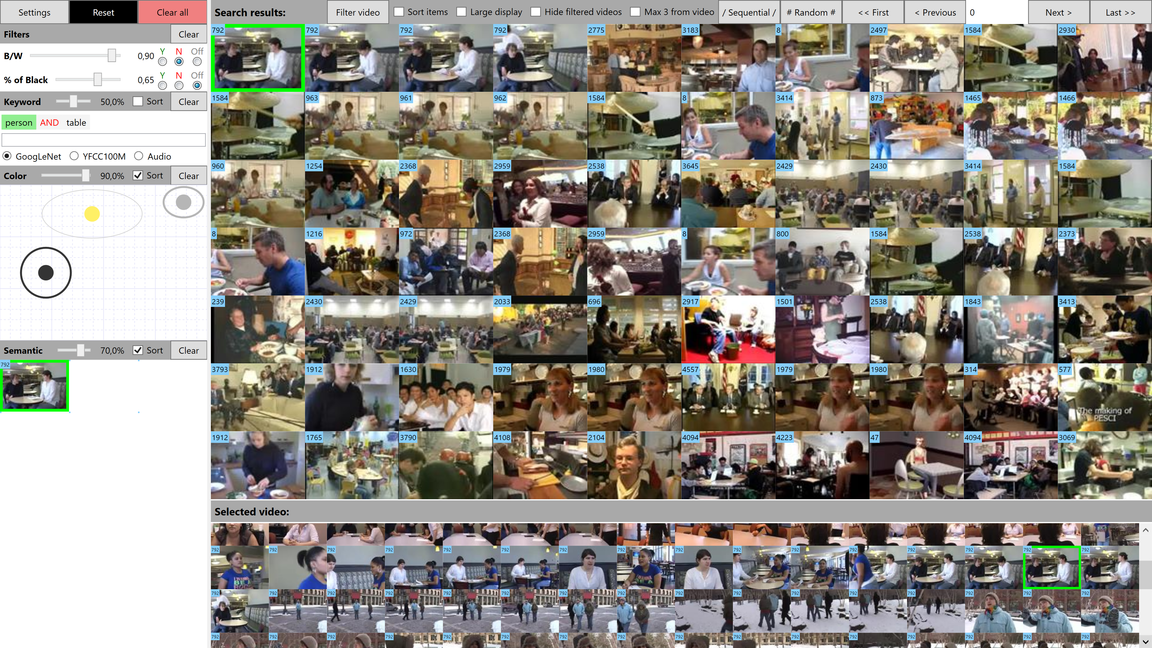
\includegraphics{img/viret_small.png}
    \caption{A sample search in VIRET framework. Source: https://videobrowsershowdown.org/hall-of-fame/}
    \label{fig:viret}
\end{figure}

\subsection{SOM Hunter}

A SOM Hunter (\cite{kratochvil2020som}) was for the first time introduced at the VBS2020. This tool is related to us, since it successfully proved using Self-organizing Maps for a use in a Known-item-search task. They train a small self-organizing map on the fly over only a sample of the dataset. This allows them to recreate the SOM based on the user interaction and train it on the fly. In our work we use the idea of training SOM, but compared to the SOM Hunter we will test creating a SOM only on the faces of the people.

\begin{figure}
    \centering
    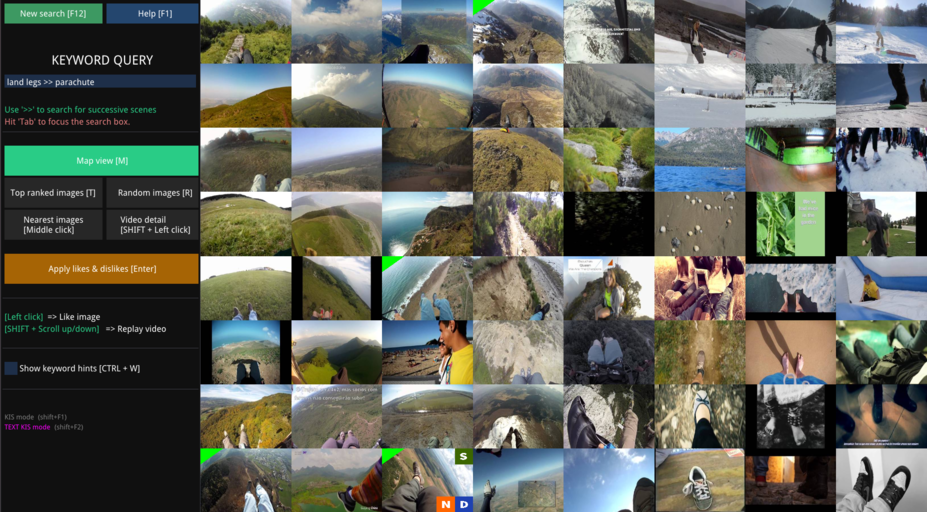
\includegraphics[width=0.99\linewidth]{img/som_hunter_small.png}
    \caption{A sample search in SOM Hunter. Source: https://videobrowsershowdown.org/hall-of-fame/}
    \label{fig:som_hunter}
\end{figure}

\subsection{Vitrivr}

Vitrivr (\cite{rossetto2016vitrivr}) is one part of more complex solution for retrieving a video in the collection. Vitrivr is the module responsive for creating queries which are then processed by the Cineast. The overview of the system is displayed in the figure \ref{fig:vitrivr}. The Vitrivr supports different query types, as query by a sketch, example image, semantic concept, keywords, audio or motion. The feature extraction and the system behind retriving the most similar results are part of the second module -- Cineast (\cite{rossetto2016searching}). Cineast uses multiple approaches incorporating deep features, i.e. scene text recognition and speech-to-text recognition. The Vitrivr (part responsible for creating the queries) is a web-browser solution, therefore the tool includes a clean separation between the query formulation and retrieving the responses.

\begin{figure}
    \centering
    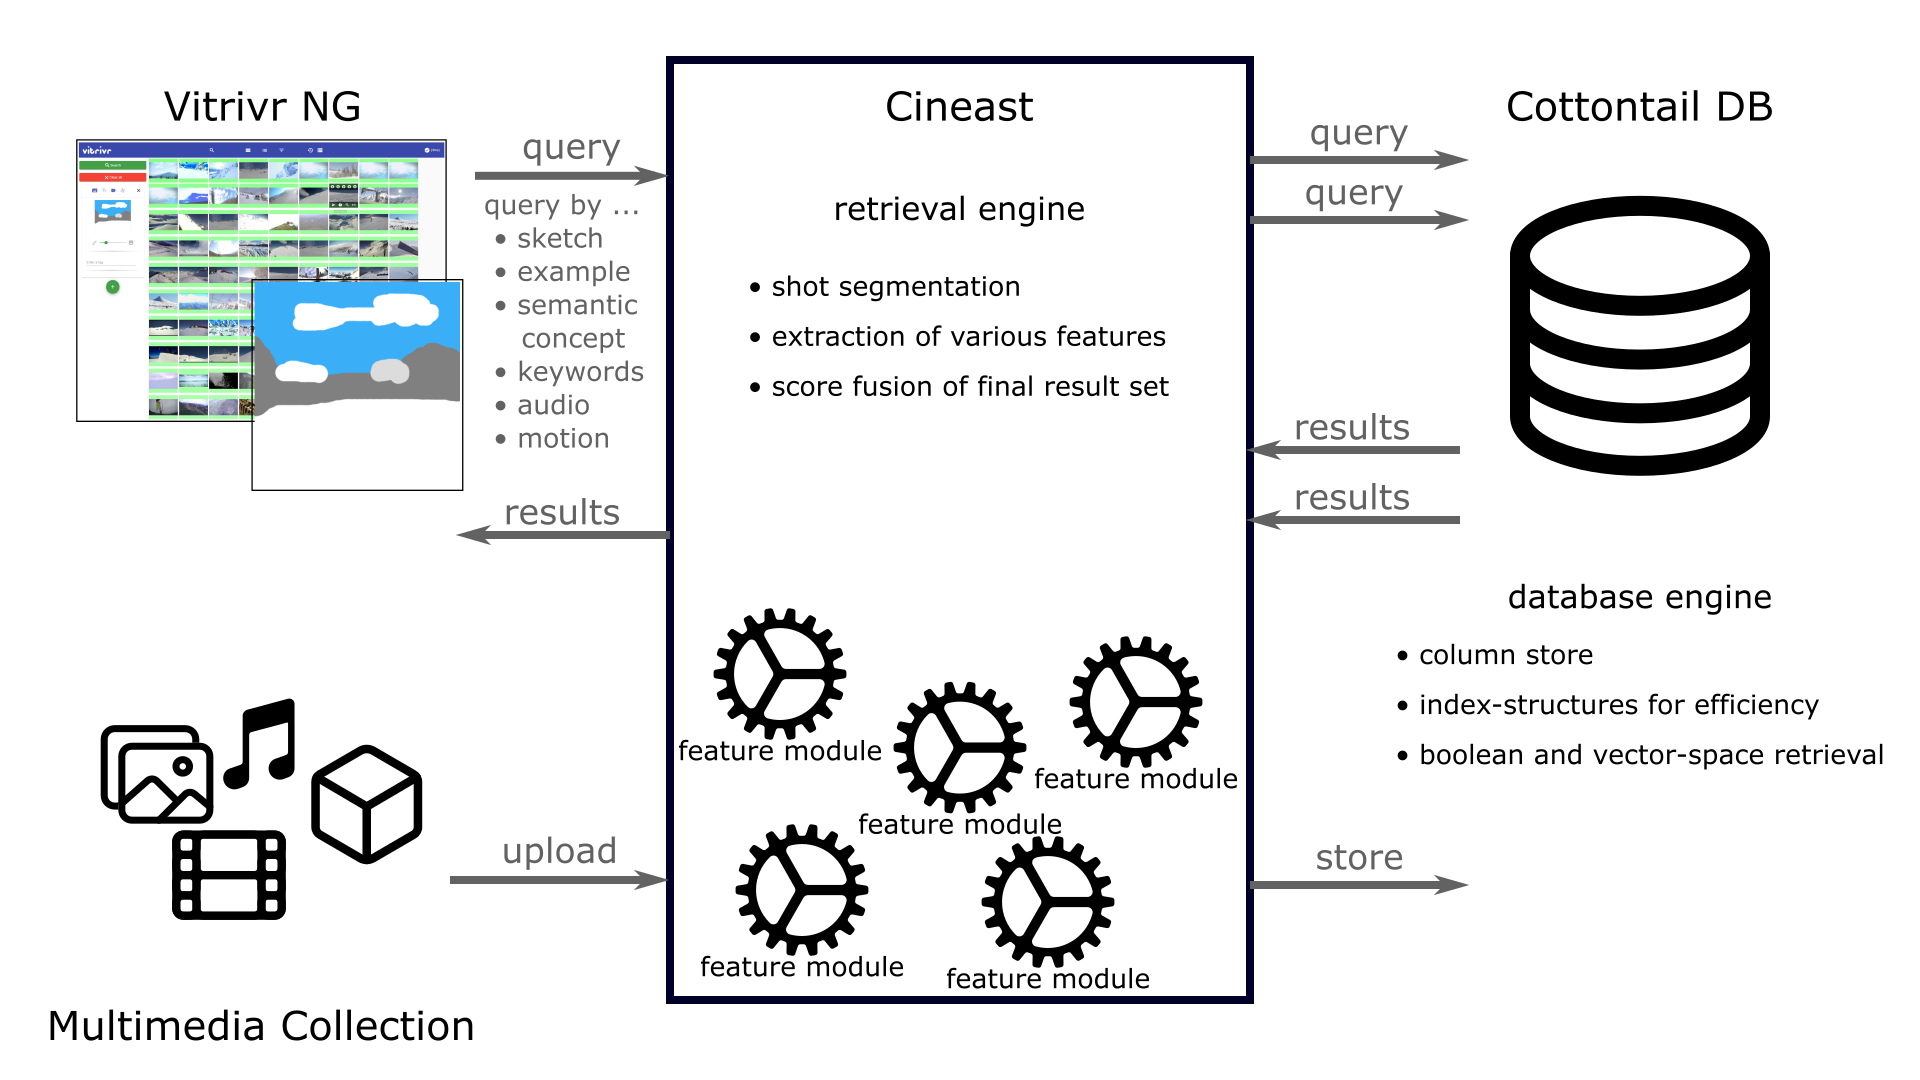
\includegraphics[width=\linewidth]{img/vitrivr.png}
    \caption{Overview of the separation in the Vitrivr solution. Source: \url{https://vitrivr.org/vitrivr.html}}
    \label{fig:vitrivr}
\end{figure}

\section{Deep Neural Networks}

In recent years we witnessed many records-breaking new machine learning models. Many of those were possible, thanks to the advancement of Deep Neural Networks (DNN). Nowadays, these models replaced more traditional Machine Learning approaches in many tasks.

Deep Neural Network is a machine learning model, whose goal is to approximate a given function \(f\). The set of parameters is often referred to as \(\theta\). One of the everyday tasks performed by these networks is classification, where the goal of the network is to predict which category sample \(X\) belongs. Even though we will not perform a classification task in this thesis, we will use some of the available classification networks.

When we talk about neural networks, we usually refer to a feedforward network. These networks consist of layers where information during the evaluation is passed only in one direction. We can imagine it as applying a function to the results from the previous layer. For example, let us create a small neural network. Denote first layer as \(f_1\) and second layer as \(f_2\). The output of the network will be \(f_2\left(f_1\left(\right)\right)\).

Stacking more and more layers on top of each other leads us to notation \emph{deep} neural networks. This notation has no fixed threshold on which networks "deserve" to be called deep. Therefore we do not recognize any importance to the naming "deep." 

The first and last layer are commonly referenced as \emph{input} and \emph{output} layer. Layers between the input and output layers are usually denoted as \emph{hidden} layers. Deep neural networks can have four or hundreds of layers, and each layer of the layer can have even a unique structure. \emph{Network Architecture} captures the "build order" of the network. It is important to note that there exist many networks with different architectures solving the same task.

There are many reasons for the advancement of neural networks in the past years. One of the crucial stones was not only theoretical innovations used for the networks but increasing computability limits. Deep Neural Networks \emph{learn} to approximate function by \emph{training}. This training is usually the heaviest part of the computation. Even though it is enough to train once and use forever, it usually lays some limitations on the size of the networks or the functions used.

Since this topic is broad, we recommend more thorough reading, such as Neural Networks and Deep learning online book\footnote{http://neuralnetworksanddeeplearning.com/}.

\subsection{Convolution Neural Networks}

Convolution Neural Networks (CNN) are a class of Deep Neural Networks. Even though they emerged in the late 1980s (\cite{lecun1989backpropagation}), it took another 20 years for further advancements in the research area. Convolution Neural Networks are mainly used in image-related tasks, such as image classification ("What is on the image?"), object detection ("Where are the objects in the image and what are they?") or even content generation ("Create a new image"). Their abilities were also tested in many, not image-related tasks, e.g., music genre recognition.

Convolution Neural Networks are specialized kind of networks which work with grid-like topology. For 1D can be an example as time-series, or for 2D, most typically image pixels represent a grid. The name \emph{convolution} refers to using a mathematical linear function \emph{convolution} in at least the layers. A simplified overview of the structure is displayed in figure \ref{fig:convolution_neural_network}. We refer to \cite{Goodfellow-et-al-2016} for more understanding of \emph{convolutional layers}.

\begin{figure}
    \centering
    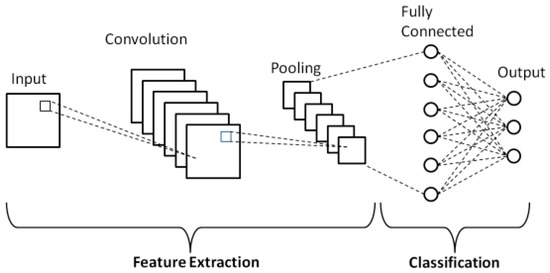
\includegraphics[width=0.98\textwidth]{img/convolution_neural_network.jpg}
    \caption{Schematic diagram of a basic convolution neural networks. Source: Phung, V.H.; Rhee, E.J. A High-Accuracy Model Average Ensemble of Convolutional Neural Networks for Classification of Cloud Image Patches on Small Datasets. Appl. Sci. 2019, 9, 4500.}
    \label{fig:convolution_neural_network}
\end{figure}

\subsection{Transfer Learning}

Transfer Learning is a research problem in machine learning that focuses on storing knowledge gained while solving one problem and applying it to a different problem. We have seen many successful transfers of the network architecture and parameters learned to a new task. Transfer learning helps to reduce the cost of the training and often also to overcome an insufficient set of training examples for the new task.

We utilize some of the pre-trained Convolution Neural Networks. The ability of a convolutional neural network to transfer to a new task by elevating gained information from other datasets was explored as early as by \cite{donahuedeep}, and many others were able to use this information to gain better models.  Networks we use are mostly pre-trained on \emph{ImageNet}\footnote{http://www.image-net.org/}. ImageNet served as a benchmark for comparing the performance of the different networks. Since the ImageNet is the main classification task, we utilize the transfer learning in a way to obtain deep features. Layers to the end of the networks accumulate more information, i.e., they contain high-level features. Therefore, we work with the layers close to the end of the networks. These layers represent encoded information about the image in high dimensional vectors. Our task is to use these deep features obtained for solving our known-search item task.


\begin{figure}
    \centering
	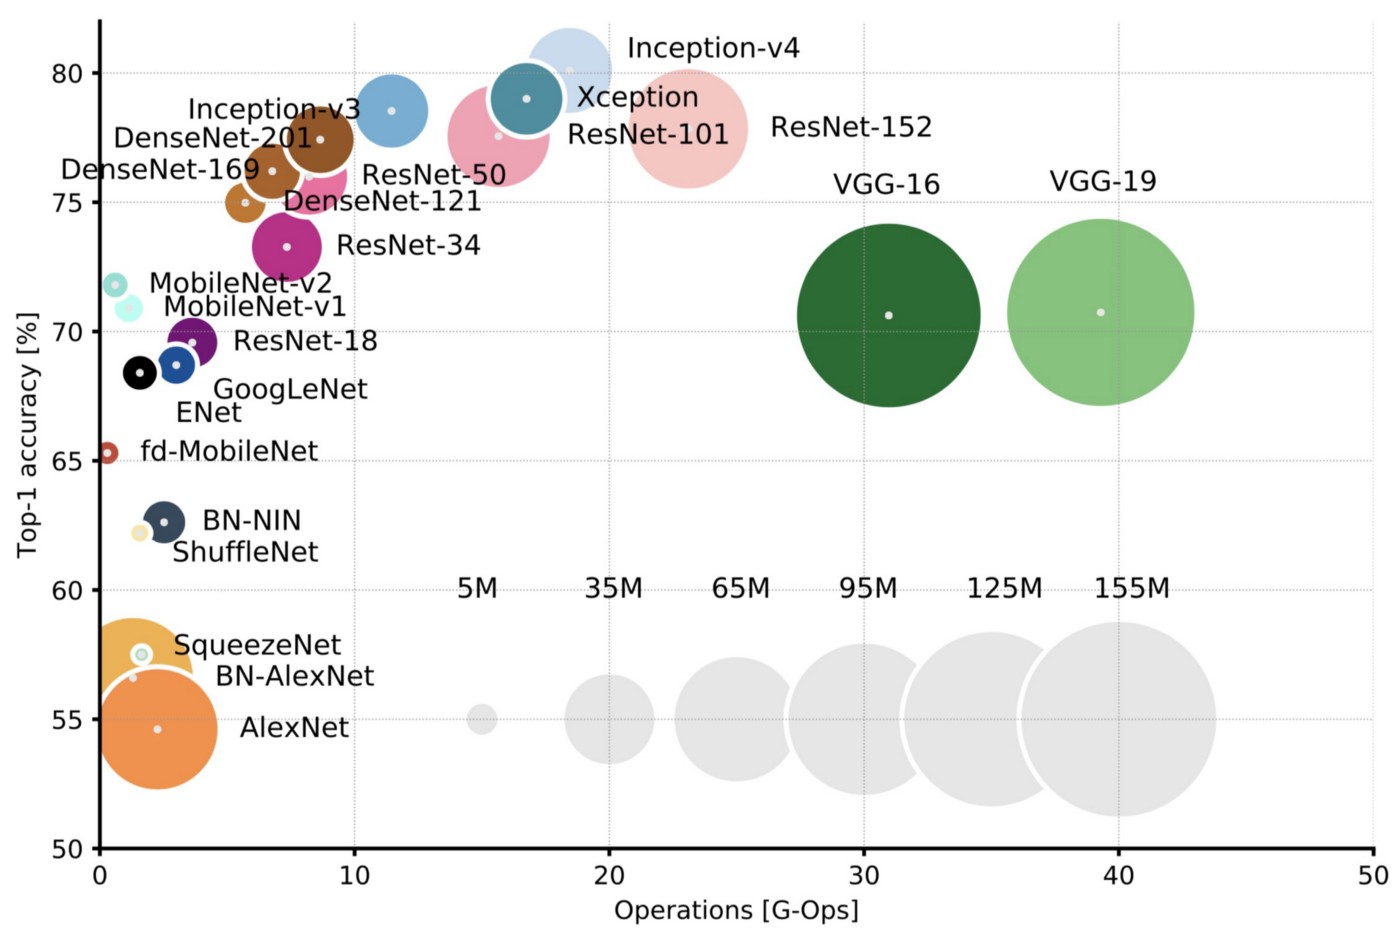
\includegraphics[width=0.8\linewidth]{img/network-comparison.jpeg}
	\caption{Top-1 one-crop accuracy versus amount of operations required for a single forward pass. The size of the blobs is proportional to the number of network parameters. Source: \cite{canziani2016analysis}}
	\label{fig:camera-setup}
\end{figure}

\subsection{Pretrained models}
\label{ss:pretrained_models}

\subsubsection{Keras}

Keras (\cite{chollet2015keras}) is a deep learning API written in Python, running on top of the machine learning platform TensorFlow\cite{tensorflow2015-whitepaper}. It was developed with a focus on experimentation in deep learning. We use it and its pre-trained models in this thesis. The models available in Keras Applications, which we use, were trained on ImageNet. Keras API allows us to separate the model from the last fully connected layer used for classification (since default ImageNet is a classification task). 

\subsection{Models Used}

\subsubsection*{Resnet50V2}
\cite{resnetv2} \cite{resnet}

\subsubsection*{MobileNetV2}
\cite{mobilenet} \cite{mobilenetv2}

\subsubsection{Dlib}
Dlib (\cite{king2009dlib}) is a modern C++ toolkit containing machine learning algorithms and tools for creating complex software in C++ to solve real-world problems. Some of the modules are provided with Python API. We use the Dlib library for face detection and also face feature extraction. For both we use face\_recognition API (\cite{geitgey2016machine}). \cite{king2017high} \todo{fix ref}







\chapter{Preliminaries}

\section{Deep Learning}

\subsection{Deep Neural Network Features}

Deep Neural Networks are composed of layers. These stacked layers on top of each other transfer sequentially information from the beginnning until the end. Several researches showed the ability of different layers percieving different type of information. The high level features are build on top of low level features, detected in the early layers. Therefore, the layers have descriptive power. Later in this thesis, we use the features from penultimate and antepenultimate layers of common image recognition Depp Neural Networks.

\begin{figure}
	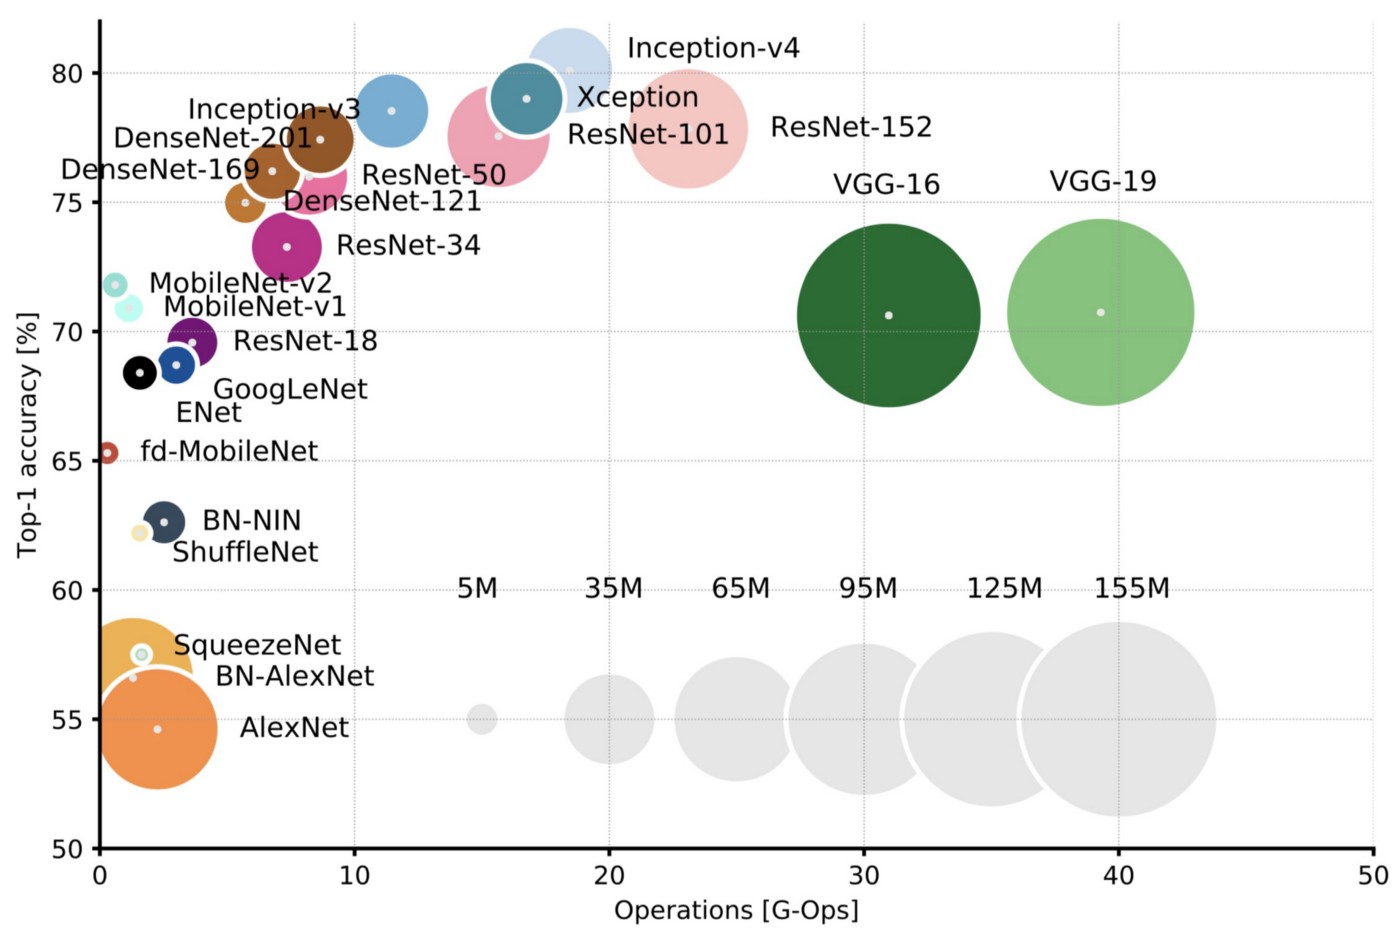
\includegraphics[width=0.8\linewidth]{img/network-comparison.jpeg}
	\caption{Comparison of widely used Image Recognition networks and their performance. Src:TODO: https://arxiv.org/abs/1605.07678}
	\label{fig:camera-setup}
\end{figure}


\section{Distance Measures}

\subsection{Cosine Distance}
\begin{equation}
similarity = \cos ({\bf t},{\bf e})= {{\bf t} {\bf e} \over \|{\bf t}\| \|{\bf e}\|} = \frac{ \sum_{i=1}^{n}{{\bf t}_i{\bf e}_i} }{ \sqrt{\sum_{i=1}^{n}{{\bf t}_i^2}} \sqrt{\sum_{i=1}^{n}{{\bf e}_i^2}} }
\end{equation}
\begin{equation}
    distance = 1 - similarity
\end{equation}

\subsection{Euclidean Distance}
\begin{equation}
d(p, q) = \sqrt{\sum_{i=1}^n (p_i - q_i)^2}    
\end{equation}

\section{Self organizing maps}

\section{?Clustering}

\section{Dataset}

\chapter{Search by Object Location}

First approach we explore is based on knowing the position of the objects in the image. This corresponds to a visual memory. People with a good visual memory are usually able to describe the position of the objects regarding to each other or in absolute way in the whole image. An example to this shows the image \todo[]{}.

We aim to overcome a limitation on vocabulary size for common approach by description of words. We implement search only on visual requests, which, if takes rich enoucgh descriptors has significantly higher capability.

\todo[inline]{Obrazok s hladanou scenou dvoch ludi a k tomu vsetkymi obrazkami kde su dvaja ludia}
\todo[inline]{Obrazok s hladanou scenou dvoch ludi a k tomu kolaz ktora zobrazuje ewquest}

\todo[inline]{Motivation --  spomienka toho, ako vyzerala scena}
\todo[inline]{Now we present following two approaches...}
In the TrackVid competition, many presented solutions are limited and do not scale well. For example is keyword search, which is limited to the size of the vocabulary. In this chapter we overcome this limitation. We develop search based on images instead of words to avoid the vocabulary limit. We use state-of-art knowledge to acquire deep representation of the objects.

The second limitation we tackle is multi-query. It is difficult to find a source video if many scenes with the same type of the objects occur in the dataset (see Image ....). We solve this problem by placing multiple single queries and then using fusion to merge rankings from each query (more in ...).


The research in the recent years showed, that neural networks purposfully trained for a set of objects can gain an ability to create a good representation also for unseen objects \todo[]{source}. In this thesis we work with this presumption and we work with these representations.

\section{Visual Descriptor}
\section{Deep Visual Representations}
--- obfuskavanie sieti

\section{Query}

The query is a collage of one or multiple images. Each image also includes its relative position in the canvas.

The user interacts with the environemnt by adding, scaling and moving images. Interactively, closest representatives found in the dataset are returned. The user can submit if he successfully found the searched scene. The number of hints are taken into account.

The image \todo[]{query image} shows an example of our query. The goal is to be able to use any of currently available image search engines to create a collage. The user places multiple images on the canvas. Their position on the canvas is recorded and later used to target the database in regard to their position. 


\section{Splitting an Image into Regions}



In our first approach we cut the image into fixed regions. We aim to capture the 
representation of each of these regions. This offers us an information specific for each region.

With the query we can compare the features representation of the query and of the particular regions we are interested in.

Image
- Split to nxm regions
- Compute deep representation for each of the regions

Query
compute deep representation for the image in the query
for each image in the database, compare this representation to the representation of the region with highest IoU


In our first approach we split the image to a regions. We compute a deep representation using neural network for each region and the whole image. 
\section{ Using Deep Representation}
   - Using Deep Representation
      = Using antepenultimate layer of classification networks

\section{Multi-query search}
- Multi query search
  - Fusion methods
  - Comparison of both approaches with multimodal performance over different fusion techniques

Our work focuses on difficult to describe scenes with multiple easy to recognize objects. In this questions a natural question of how to rank the results based on multi query.

In this section we go through several approaches we tested. We base our 

\subsection{Fusion Methods}

\section{Evaluation}
In this chapter we evaluate all previously mentioned approached. Firstly, we describe our methodology behind the experiments and then we proceed through all approaches. 

\chapter{Search by Face Similarity}

Research in past several decades proved that human have extreme capability of recognizing the faces. Faces are so special to us as a species, that we are able to ..... We are able to recall that we met specific person dating the meeting years back. Therefore we state a question, if the search based only on faces can be done.

This approach organizes the space of seen faces to help the user to orientate and find the search face. Though, in order to describe the face space we use deep encodings trained by a network used for face recognition.

In the previous chapter we elaborated an approach to search in dataset using objects and their spatial information. In this chapter we investigate a different option -- traversion using faces. The question we ask is if it is possible to find a specific scene by showing user faces. Since there is a limitation of how many faces we can display at once to the user, we will investigate if we can lead user to the specific scene with specific face via traversion through multiple similar faces.

Since the similarity of faces is a strongly abstract perception we rely on feature representation of the faces. This helps us to create an interactive environment to traverse via huge aount of faces and test our hypothesis, if this approach can be used for scene searching. 

This chapter firstly introduces different approaches to obtaining face representations. Then we proceed by presenting different approaches for traversion over dataset of faces. At the end of the chapter we present the results in our specific task -- scene search .

\todo[inline]{ motivation - otestovat hypotezu ci je to mozne a nejaky nahlad ako ot moze vyzerat}
\section{Preliminaries}
\todo[inline]{face features - popisat zdroj siete}
\section{Creating SOM Representation of the face space}
\section{Evaluation}

Appendix
\chapter{User Guide (how to use the app to search)}
\chapter{ Running the app on the new set of images}
\todo[inline]{kde zmenit data a co znova natrenovat}
\chapter{Experiments evaluation (ako ziskat vysledky znova)}
\chapter{Code Structure (programmer's guide)}


% Searching Image Collections Using Deep Representations of Local Regions

% The thesis will investigate two particular approaches for searching large video datasets. The first approach will try to retrieve a searched scene based on a query collage consisting of example images organized on a canvas. The author will investigate various fusion methods, taking into account also the canvas positioning of the query images.  The second approach will be designed to search for a scene based on faces available in the dataset. The method will be based on visual exploration of the faces based on their similarities. In exploration approaches, the user can choose a similar face to the searched one, and continuously browse towards the searched face. The author will provide an interactive search environment for querying as a part of the solution and evaluate the recall on sets of experiments to estimate, how successfully users can retrieve particular scenes.


% \chapter{Title of the second chapter}

\section{Title of the first subchapter of the second chapter}

\section{Title of the second subchapter of the second chapter}


\chapter*{Conclusion}
\addcontentsline{toc}{chapter}{Conclusion}


%%% Bibliography
%%% Bibliography (literature used as a source)
%%%
%%% We employ bibTeX to construct the bibliography. It processes
%%% citations in the text (e.g., the \cite{...} macro) and looks up
%%% relevant entries in the bibliography.bib file.
%%%
%%% The \bibliographystyle command selects, which style will be used
%%% for references from the text. The argument in curly brackets is
%%% the name of the corresponding style file (*.bst). Both styles
%%% mentioned in this template are included in LaTeX distributions.

\bibliographystyle{plainnat}    %% Author (year)
% \bibliographystyle{unsrt}     %% [number]

\renewcommand{\bibname}{Bibliography}

%%% Generate the bibliography. Beware that if you cited no works,
%%% the empty list will be omitted completely.

\bibliography{bibliography}

%%% If case you prefer to write the bibliography manually (without bibTeX),
%%% you can use the following. Please follow the ISO 690 standard and
%%% citation conventions of your field of research.

% \begin{thebibliography}{99}
%
% \bibitem{lamport94}
%   {\sc Lamport,} Leslie.
%   \emph{\LaTeX: A Document Preparation System}.
%   2nd edition.
%   Massachusetts: Addison Wesley, 1994.
%   ISBN 0-201-52983-1.
%
% \end{thebibliography}


%%% Figures used in the thesis (consider if this is needed)
\listoffigures

%%% Tables used in the thesis (consider if this is needed)
%%% In mathematical theses, it could be better to move the list of tables to the beginning of the thesis.
\listoftables

%%% Abbreviations used in the thesis, if any, including their explanation
%%% In mathematical theses, it could be better to move the list of abbreviations to the beginning of the thesis.
\chapwithtoc{List of Abbreviations}

%%% Attachments to the master thesis, if any. Each attachment must be
%%% referred to at least once from the text of the thesis. Attachments
%%% are numbered.
%%%
%%% The printed version should preferably contain attachments, which can be
%%% read (additional tables and charts, supplementary text, examples of
%%% program output, etc.). The electronic version is more suited for attachments
%%% which will likely be used in an electronic form rather than read (program
%%% source code, data files, interactive charts, etc.). Electronic attachments
%%% should be uploaded to SIS and optionally also included in the thesis on a~CD/DVD.
%%% Allowed file formats are specified in provision of the rector no. 72/2017.
\appendix
\chapter{Attachments}

\section{First Attachment}

\openright
\end{document}
